\documentclass{article}

% Packages for better formatting and math support
\usepackage{amsmath}
\usepackage{graphicx}
\usepackage{hyperref}
\usepackage{listings}
\usepackage{geometry}
\usepackage{authblk}

% Adjust margins
\geometry{margin=0.8in}

% Title information
\title{CS456 Assignment 3: Part C}
\author{Jiaze Xiao}
\affil{20933691}
\date{\today}

\begin{document}

\maketitle

\section*{Question 1}
\textbf{Answer:}
\begin{quote}
    When initiating a ping from \texttt{h1} to \texttt{h5} using the command \texttt{h1 ping h5} in Mininet, the POX controller automatically handles the packet forwarding. Here is a screenshot of the output in the POX controller terminal:

    \begin{center}
        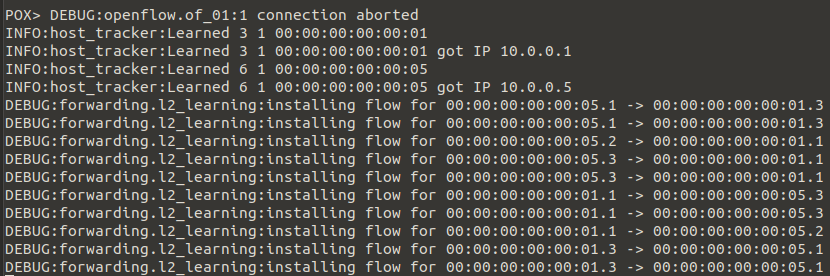
\includegraphics[scale=0.7]{screenshot/pox.png}
    \end{center}

    The \texttt{host\_tracker} module of the POX controller logs indicate that the controller has learned about the existence of hosts in the network. Specifically, it learns about hosts \texttt{h1} and \texttt{h5} along with their corresponding MAC addresses and IP addresses.

    The \texttt{forwarding.l2\_learning} module is responsible for installing flow rules in the switches. The logs show multiple `DEBUG` entries indicating the installation of flows for specific MAC addresses. Each installed flow represents a path that packets will take between \texttt{h1} and \texttt{h5}. The paths are determined based on the learned MAC addresses and the shortest path in the network topology.

    In this topology, a tree structure is used where switches are interconnected and hosts are connected to switches. The path packets take from \texttt{h1} to \texttt{h5} involves multiple switches (\texttt{s3, s2, s1, s5, s6}). For each pair of source and destination MAC addresses, the controller installs bidirectional flows to ensure connectivity. The number of logs correlates with the number of flows needed to establish the connection through the intermediate switches.
\end{quote}
\newpage
\section*{Question 2}
\textbf{Answer:}
\begin{quote}
    \begin{center}
        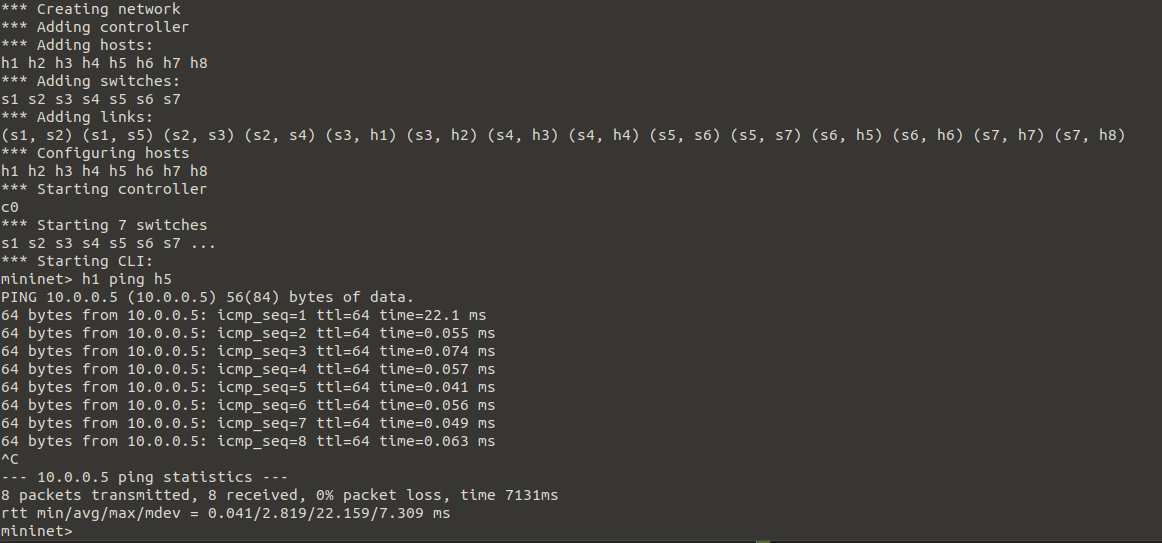
\includegraphics[scale=0.5]{screenshot/ping.png}
    \end{center}

    From the screenshot, the RTT for the first ping message is 22.1 ms and the RTTs for the subsequent ping messages are significantly lower (within 0.1ms).

    There is a noticeable difference between the RTT of the first ping message and the RTTs of the subsequent ones. When the first ping message is sent from \texttt{h1} to \texttt{h5}, the switches along the path do not have any flow rules installed for this traffic. This process of sending the packet to the controller, computing the path, and installing flow rules introduces additional delay, resulting in a higher RTT for the first ping message. After the flow rules have been installed by the controller, the subsequent ping messages follow these pre-established paths. This results in much lower RTTs for the subsequent ping messages, as the additional delay from controller involvement is no longer present.
\end{quote}
\newpage
\section*{Question 3}
\textbf{Answer:}
\begin{quote}
    Flow rules before ping:
    \begin{center}
        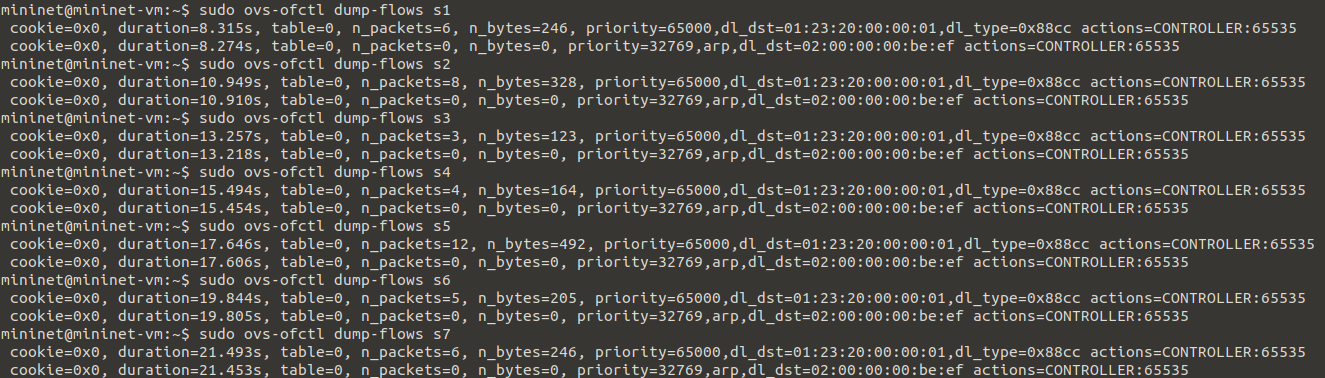
\includegraphics[scale=0.44]{screenshot/dump-flow-before.png}
    \end{center}
    Flow rules after ping:
    \begin{center}
        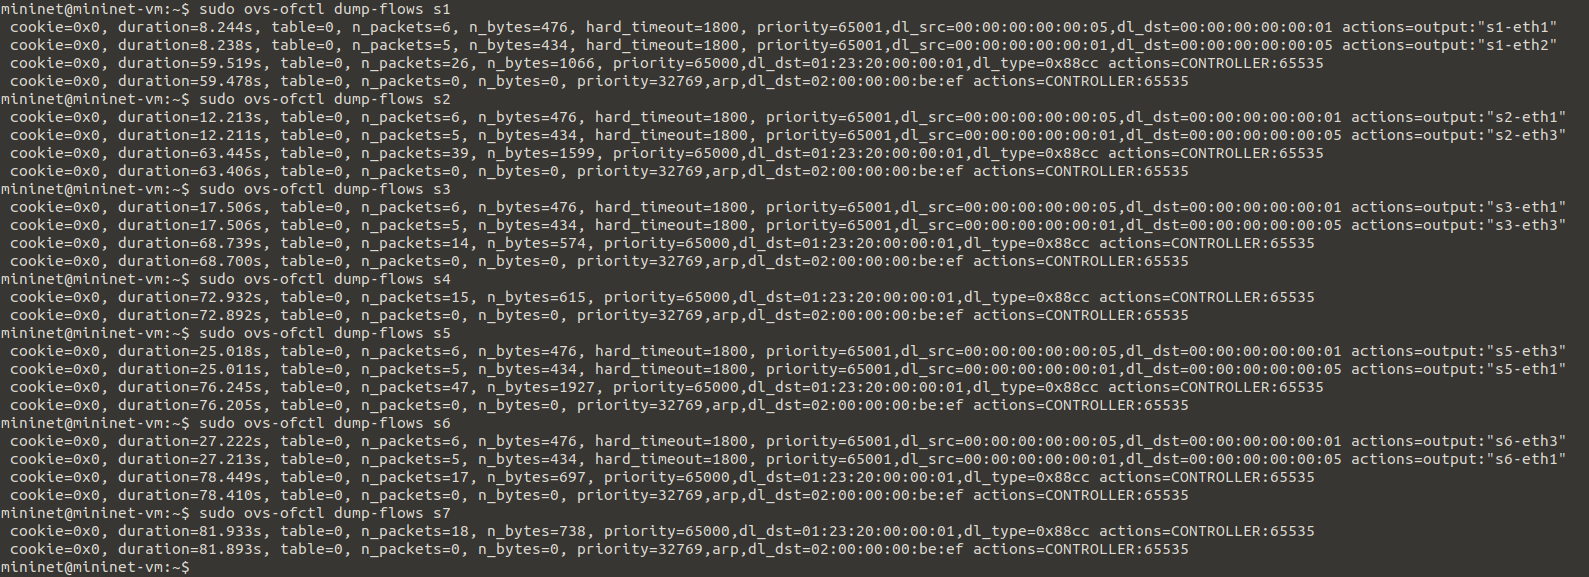
\includegraphics[scale=0.375]{screenshot/dump-flow-after.png}
    \end{center}

    From the screenshot of flow rules before ping, every switch has two rules. The initial rules in each switch are primarily for handling ARP packets. These rules ensure that ARP requests and responses are sent to the controller to learn the MAC addresses of hosts.

    After the ping command is executed, additional flow rules are installed in \texttt{s1, s2, s3, s5, s6} which are switches on the path from \texttt{h1} to \texttt{h2}. These rules have higher priority, ensuring efficient forwarding of packets.

    These observations indicate that the controller dynamically manages the network by installing specific flow rules as needed.
\end{quote}

\end{document}
